\documentclass[11pt]{mwart}
\usepackage{tocloft}
\usepackage[polish]{babel}
\usepackage[utf8]{inputenc}
\usepackage{float}
\usepackage{enumerate}
\usepackage{listings}
\usepackage{subfig}
\usepackage{graphicx}
\usepackage{mathpazo}
%\usepackage{times}
%\usepackage{lmodern}
%\usepackage{bera}
\usepackage[T1]{fontenc}
\usepackage{color}

\definecolor{matlabgreen}{rgb}{0, 0.7, 0}
\definecolor{matlabblue}{rgb}{0, 0, 0.7}
\definecolor{matlabred}{rgb}{1, 0, 0}

\usepackage{booktabs}
\usepackage{amsfonts}
\usepackage{amsmath}

\usepackage{geometry}
\geometry{verbose,tmargin=2.5cm,bmargin=2.5cm,lmargin=2.5cm,rmargin=2.5cm}

\usepackage[
        unicode=true,
        bookmarks=true,
        bookmarksnumbered=false,
        bookmarksopen=false,
        breaklinks=false,
        pdfborder={0 0 1},
        backref=false,
        colorlinks=false]{hyperref}
		
\hypersetup{
        pdftitle={Sterowanie optymalne - wahadło reakcyjne},
        pdfauthor={Kajetan Świerk}}

\linespread{1.15}
\lstloadlanguages{TeX}

% Ustawienia parametrow rozdzialow
\usepackage{titlesec}
\usepackage{titletoc}

\titleformat{\section}
{\bfseries\Large}{\filright \Large\thesection. }{0ex}{}
\titlespacing{\section}{7mm}{8mm plus 0mm minus 1mm}{4mm plus 0mm minus 1mm}

\renewcommand{\cfttoctitlefont}{\bfseries\Large}
\renewcommand{\cftbeforetoctitleskip}{20mm}
\renewcommand{\cftaftertoctitleskip}{19mm}
\renewcommand{\cftsecleader}{\cftdotfill{\cftdot}}
\renewcommand{\cftsubsecleader}{\cftdotfill{\cftdot}}
\renewcommand{\cftsecaftersnum}{.}
\setlength{\cftparskip}{2pt}

\begin{document}

\author{Piotr Binduga, Kajetan Świerk}
\title{\Huge{Wahadło reakcyjne} \\ \vspace{0.2cm} \small{Optymalizacja w systemach sterowania}}

\maketitle
\tableofcontents{}
\newpage{}

\section{Sformułowanie problemu}
Celem projektu jest doprowadzenie wahadła reakcyjnego do górnej pozycji startując z~pozycji dolnej za pomocą wyznaczonego sterowania czasooptymalnego. 

\section{Model obiektu}
Model wahadła reakcyjnego można opisać za pomocą równań
\begin{equation}
	\begin{split}
		J\ddot{x}_{q1} &=  mgl\sin\left({x_{q1}}\right)-ku \\
		J_{r}\ddot{x}_{q2} &= ku
	\end{split}
\end{equation}
gdzie:

\noindent\begin{minipage}[t]{0.75\columnwidth}
	$J=J_{p}+m_{p}l_{p}^{2}+m_{r}l_{r}^{2}$ \\
	$J_{p}$ - moment bezwładności wahadła \\
	$m_{p}$ – masa wahadła \\
	$m_{r}$ – masa koła \\
	$l_{p}$ – długość wahadła \\
	$l_{r}$ - odległość od osi obrotu do środka masy wahadła \\
	$J_{r}$ - moment bezwładności koła \\
	$\ddot{x}_{q1}$ - przyspieszenie kątowe wahadła \\
	$\ddot{x}_{q2}$ - przyspieszenie kątowe koła\\
	$m$ - masa wahadła wraz~z~kołem\\
	$l$ - odległość od osi obrotu do środka masy wahadła wraz~z~kołem \\
	$k$ - stała momentu obrotowego silnika DC \\
	$u$ - sterowanie
\end{minipage}
\begin{minipage}[t]{0.25\columnwidth}
	% \begin{equation*}
		% \begin{split}
			% J&=0,004572\ \textrm{kgm}^2 \\
			% J_{p}&=0,0002233\ \textrm{kgm}^2 \\
			% m_{p}&=-0,2164\ \textrm{kg} \\
			% m_{r}&=0,085\ \textrm{kg} \\
			% l_{p}&=0,1173\ \textrm{m} \\
			% l_{r}&=0,127\ \textrm{m} \\
			% J_{r}&=0,00002495\ \textrm{kgm}^2
		% \end{split}
	% \end{equation}
	$J=0,004572\ \textrm{kgm}^2$ \\
	$J_{p}=0,0002233\ \textrm{kgm}^2$ \\
	$m_{p}=-0,2164\ \textrm{kg}$ \\
	$m_{r}=0,085\ \textrm{kg}$ \\
	$l_{p}=0,1173\ \textrm{m}$ \\
	$l_{r}=0,127\ \textrm{m}$ \\
	$J_{r}=0,00002495\ \textrm{kgm}^2$ \\
	\\
	\\
	$m=0,3014\ \textrm{kg}$ \\
	$l=0,12\ \textrm{m}$\\
	$k=0,0274\ \textrm{Nm/A}$ \\
	\\
\end{minipage}

\begin{figure}[ht]
	\begin{centering}
	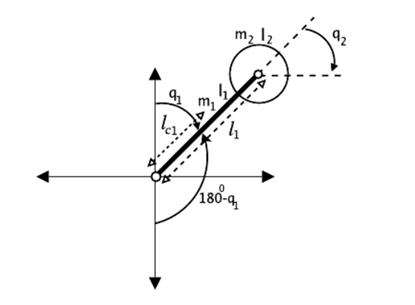
\includegraphics[scale=1.0]{model}
	\caption{Schemat wahadła reakcyjnego.}
	\label{fig-model}
	\end{centering}
\end{figure}

Przyjmując następujące zmienne stanu:
\begin{equation}
	\label{eq-rowstanu}
	\begin{split}
		x_{1} &= x_{q1} \\
		x_{2} &= \dot{x}_{q1} \\
		x_{3} &= x_{q2} \\
		x_{4} &= \dot{x}_{q2}
	\end{split}
\end{equation}

równania stanu (\ref{eq-rowstanu}) prezentują się następująco:

\begin{equation}
	\label{eq-rowstanu1}
	\begin{split}
		\dot{x}_{1} &= x_2 \\
		\dot{x}_{2} &= \frac{mgl}{J}\sin\left(x_{1}\right)-\frac{k}{J}u \\
		\dot{x}_{3} &= x_{4} \\
		\dot{x}_{4} &= \frac{k}{J_{r}}u
	\end{split}
\end{equation}

\section{Zadanie sterowania}

Zadaniem sterowania jest osiągnięcie górnego położenia równowagi tj. $x^f=[0\ 0\ \alpha\ 0]^T$, $\alpha\in~\mathbb{R}$ w jak najkrótszym czasie $t_f$. W tym celu definiujemy pomocnicze zadania optymalności przy ustalonym horyzoncie czasowym $T\geq0$. Dla określonego $T$ pomocniczy funkcjonał jakości wyraża się za pomocą

\begin{equation}
	\label{eq-wskjakosci}
	\begin{split}
		Q_{T}\left(u\right) &= \frac{1}{2}\left(x\left(T\right)-x^f\right)R\left(x\left(T\right)-x^f\right) \\
		Q_{T}\left(u\right) &= q\left(x\left(T\right)\right)
	\end{split}
\end{equation}

gdzie macierz~$R=R^T>0$. Zbiór wartości optymalnych $Q_T$ oznaczymy przez~$\sum\left(T\right)$. Poszukiwany horyzont minimalny spełnia zależność

\begin{equation}
	t_{f}=\min\left\{T:\sum\left(T\right)=0\right\}
\end{equation}

Na sterowanie nałożone jest ograniczenie 

\begin{equation}
	\left|u\left(t\right)\right|\leq 1
\end{equation}

\newpage{}

\section{Całkowanie równań stanu}

Do rozwiązania równań systemu zastosowano metodę Rungego-Kutty 4. rzędu z~krokiem~$h$

\begin{equation}
	\begin{split}
		x_{i+1} &= x_{i} + \frac{1}{6}\cdot\left(k_{1}+2k_{2}+2k_{3}+k_{4}\right) \\
		k_{1} &= h\cdot f\left(x_{i},u_{i}\right) \\
		k_{2} &= h\cdot f\left(x_{i}+\frac{1}{2}k_{1},u_{i}\right) \\
		k_{3} &= h\cdot f\left(x_{i}+\frac{1}{2}k_{2},u_{i}\right) \\
		k_{4} &= h\cdot f\left(x_{i}+k_{3},u_{i}\right) \\
	\end{split}
\end{equation}


gdzie $f\left(x\left(t\right),u\left(t\right)\right)$ to prawa strona równania systemu (\ref{eq-rowstanu1}). Warto zaznaczyć, że sterowanie w danym przedziale całkowania jest stałe i dlatego dla każdego $k_{n}$ po prawej stronie równania występuje $u_{i}$.

\section{Zastosowanie zasady maksimum Pontyagrina}

Hamiltonian przyjmuje postać

\begin{equation}
	\label{eq-ham}
	\begin{split}
		H &= \Psi^Tf\left(x\left(t\right),u\left(t\right)\right) \\
		H &= \Psi_{1}\left(t\right)x_{2}\left(t\right) + 
		\Psi_{2}\left(t\right)\frac{mgl}{J}\sin\left(x_{1}\left(t\right)\right) +\\
		& \Psi_{3}\left(t\right)x_{4}\left(t\right) +
		u\left(t\right)\left[-\Psi_{2}\left(t\right)\frac{k}{J}+\Psi_{4}\left(t\right)\frac{k}{J_{r}}\right] \\
		H &= \Psi^Tf^0\left(x\left(t\right)\right)+\Psi^Tf^1\left(x\left(t\right)\right)u\left(t\right)
	\end{split}
\end{equation}

gdzie $\Psi\left(t\right)$ jest rozwiązaniem równania sprzężonego

\begin{equation}
	\label{eq-rowsprz}
	\begin{split}
		\dot{\Psi}\left(t\right) &= -\frac{\partial H}{\partial x} \\
		\Psi\left(T\right) &= -\frac{\partial q}{\partial x\left(T\right)}
	\end{split}
\end{equation}

\begin{equation}
	\label{eq-rowsprz1}
	\begin{split}
		\dot{\Psi}_{1}\left(t\right) &= -\frac{\partial H}{\partial x_{1}} = -\Psi_{2}\left(t\right)\frac{mgl}{J}\cos\left(x_{1}\left(t\right)\right) \\
		\dot{\Psi}_{2}\left(t\right) &= -\frac{\partial H}{\partial x_{2}} = -\Psi_{1}\left(t\right) \\
		\dot{\Psi}_{3}\left(t\right) &= -\frac{\partial H}{\partial x_{3}} = 0 \\
		\dot{\Psi}_{4}\left(t\right) &= -\frac{\partial H}{\partial x_{4}} = -\Psi_{3}\left(t\right) \\
		\Psi\left(T\right) &= -R\cdot\left(x^f-x\left(T\right)\right)
	\end{split}
\end{equation}

Równania (\ref{eq-rowsprz1}) całkowane są wstecz, zaczynając od chwili końcowej, co wynika wprost z~danych warunków końcowych na $\Psi\left(T\right)$.

Zgodnie z~teorią Hamiltonian dla trajektorii sprzężonej optymalnej, trajektorii optymalnej oraz~sterowania optymalnego przyjmuje maksymalną wartość w każdej chwili czasu.

\begin{equation}
	H\left(\Psi\left(t\right),x\left(t\right),u\left(t\right)\right)\geq H\left(\Psi\left(t\right),x\left(t\right),v\left(t\right)\right),\ \forall v\in D
\end{equation}

\section{Postać sterowania}

Z~postaci Hamiltonianu wynika, iż sterowaniem optymalnym jest sterowanie typu Bang-bang, tj. leżące na ograniczeniach. Sterowanie takie określone jest jednoznacznie poprzez~parę $\{u_{0},\tau\}$, gdzie $\tau=\{\tau_{1},\tau_{2},\dots,\tau_{n}\}$ wyznacza czasy, w których następuję przełączenie sterowanie na inne ograniczenie. 
Dla ustalonej liczby czasów przełączeń $n$, optymalizację prowadzić będziemy w przestrzeni o wymiarze równym $n$. W przestrzeni tej gradient, tj. pochodna wskaźnika jakości względem czasów przełączeń wynosi

\begin{equation}
	\frac{dq}{d\tau}=\left[
	\begin{array}{c}
		\frac{dq}{d\tau_{1}} \\
		\vdots \\
		\frac{dq}{d\tau_{n}}
	\end{array}
	\right]
\end{equation}

gdzie

\begin{equation}
	\frac{dq}{d\tau_{i}} = \varphi\left(\tau_{i}\right)\left(u\left(\tau_{i}^{+}\right)-u\left(\tau_{i}^{-}\right)\right)
\end{equation}

natomiast $\varphi\left(t\right)$ to tzw. funkcja przełączająca, określona jako

\begin{equation}
	\varphi\left(t\right)=\Psi^{T}f^{1}\left(x\left(t\right)\right)=-\Psi_{2}\left(t\right)\frac{k}{J}+\Psi_{4}\left(t\right)\frac{k}{J_{r}}
\end{equation}

\section{Weryfikacja pochodnej wskaźnika jakości względem czasów przełączeń}

W celu dokonania weryfikacji przeprowadzono prosty eksperyment. Dla danego czasu przełączenia zaburzono chwilę jego wystąpienia o $\varepsilon$. Za pomocą klasycznego wzoru na iloraz~różnicowy porównano wynik dla rosnącego $\varepsilon$ z~pochodną wyliczoną w poprzednim rozdziale.

\begin{equation}
	\frac{dq}{d\tau_{1}}=\lim_{\varepsilon\rightarrow0}\frac{Q_{T}\left(\tau_{1}+\varepsilon\right)-Q_{T}\left(\tau_{1}\right)}{\varepsilon}
\end{equation}

\pagebreak
Uzyskany wynik dla $\tau_{1}=2$ oraz~$T=4$ pokazano na rysunku \ref{fig-werpochodna}. Jak widać, przy malejącej wartości odchyłki $\varepsilon$ wartość ilorazu różnicowego zmierza do wartości pochodnej, co było do pokazania.

\begin{figure}[H]
	\begin{centering}
	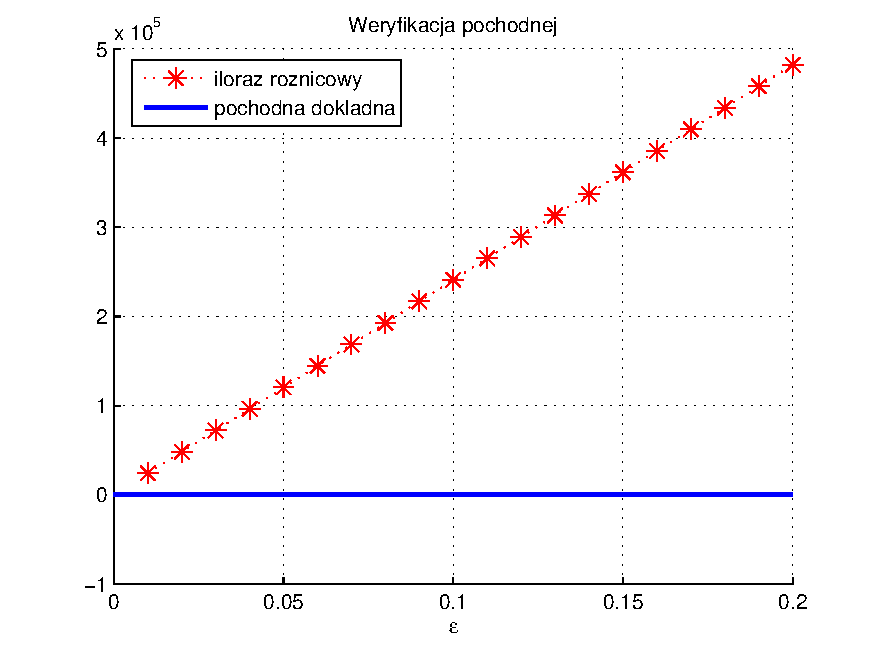
\includegraphics[scale=1.0]{pochodna}
	\caption{Weryfikacja pochodnej dla przyjętego czasu przełączeń.}
	\label{fig-werpochodna}
	\end{centering}
\end{figure}

\section{Optymalizacja w przestrzeni czasów przełączeń}

Dla danej struktury sterowania przeprowadzana jest optymalizacja za pomocą algorytmu quasi-newtonowskiego BFGS. Kierunek poszukiwania $d$ na prostej wyznacza się z równania 
\begin{equation}
	W_{k}d=-\nabla Q\left(\tau_{k}\right)
\end{equation}

$W_{k}$ uzyskuje się na drodze iteracyjnej:

\begin{equation}
	\label{eq-bfgs}
	\begin{split}
		W_{1} &= I \\
		W_{k+1} &= W_{k} + \frac{rr^{T}}{r^{T}s}-\frac{W_{k}ss^{T}W_{k}}{s^{T}W_{k}s} \\
	\end{split}
\end{equation}

gdzie:

\begin{equation}
	\label{eq-rs}
	\begin{split}
		r &= \nabla Q\left(\tau_{k+1}\right)-\nabla Q\left(\tau_{k}\right) \\
		s &= \tau_{k+1} - \tau_{k}
	\end{split}
\end{equation}

Czas przełączenia $\tau_{i}$ przesunięty na kierunku $d_{i}$ o $\alpha$ oznaczymy jako
\begin{equation}
	\tau_{i}\left(\alpha\right)=\tau_{i}\left(0\right)+\alpha d_{i}
\end{equation}

Z nierówności $\tau_{i}\leq\tau_{i+1}$ uzyskujemy
\begin{equation}
	\alpha\cdot\left(d_{i}-d_{i+1}\right)\leq\tau_{i+1}\left(0\right)-\tau_{i}\left(0\right)
\end{equation}
\begin{equation}
	\alpha_{max} = \min\left\{\frac{\tau_{i+1}\left(0\right)-\tau_{i}\left(0\right)}{d_{i}-d_{i+1}},\ d_{i}-d_{i+1}>0\right\}
\end{equation}

Wynika z tego, że metoda poszukiwania na kierunku musi zostać zmodyfikowana tak, aby uniemożliwić zamianę kolejności czasów przęłączeń a także opuszczenie przez nich przedziału czasu $[0,T]$. W pierwszej kolejności sprawdzana jest wartość $Q_{T}$ dla maksymalnego dopuszczalnego kroku a później, jeśli jest ona gorsza od obecnie najlepszej, wykonywana jest kilkuiteracyjna kontrakcja na półprostej.

Ponadto, po każdej procedurze poszukiwania na kierunku wykonywana jest redukcja czasów przełączeń w sytuacji gdy $\tau_{i}=\tau_{j},i\neq j$ lub gdy $\tau_{i}$ należy do zbioru $\left\{0,T\right\}$. Pomyślne zastosowanie redukcji zmienia strukturę sterowania przez co konieczna jest odnowa macierzy~$W_{k}$.

Po zakończeniu poszukiwania wartości optymalnej w danej strukturze sterowania, porównywana jest funkcja przełączająca $\varphi\left(t\right)$ ze sterowaniem $u\left(t\right)$. W miejscu największej efektywności $E_{max}$, określonej wzorem (\ref{eq-eff}) wprowadzana jest nowa para przełączeń. Jeśli $E_{max}$ osiągany jest dla końców przedziału czasu, wprowadzane jest tylko jedno przełączenie. 

\begin{equation}
	\label{eq-eff}
	E_{max} = \min_{t\in\left[0,T\right]} u\left(t\right)\cdot\varphi\left(t\right)
\end{equation}

Następnie algorytm BFGS uruchamiany jest z powrotem. W przypadku gdy $E_{max}$ jest bliskie zeru (przyjęto $10^{-6}$) oznacza to, że dla danego horyzontu sterowanie optymalne zostało znalezione - sprowadza się to do zgodności znaków funkcji $\varphi\left(t\right)$ i $u\left(t\right)$ w całym rozpatrywanym przedziale czasowym.

\pagebreak

\section{Wyniki optymalizacji dla różnych horyzontów czasowych}

Dla wszystkich zadań pomocniczych przyjęto macierz wagową funkcjonału jakości równą
\[
	R = \left[
	\begin{array}{cccc}
	50 & 0 & 0 & 0 \\
	0 & 50 & 0 & 0 \\
	0  & 0 & 0 & 0 \\
	0  & 0 & 0 & 1
	\end{array}
	\right]
\]

Na rysunkach (\ref{fig-ex1}) i (\ref{fig-ex2}) przedstawiono przykładowe przebiegi dla sterowania optymalnego (w sensie pomocniczego wskaźnika jakości) w zależności od przyjętego horyzontu czasowego~$T$.

\begin{figure}[H]
	\begin{centering}
	\subfloat[Przebieg pozycji ({\color{matlabblue}niebieski}) oraz prędkości ({\color{matlabgreen}zielony}) wahadła]{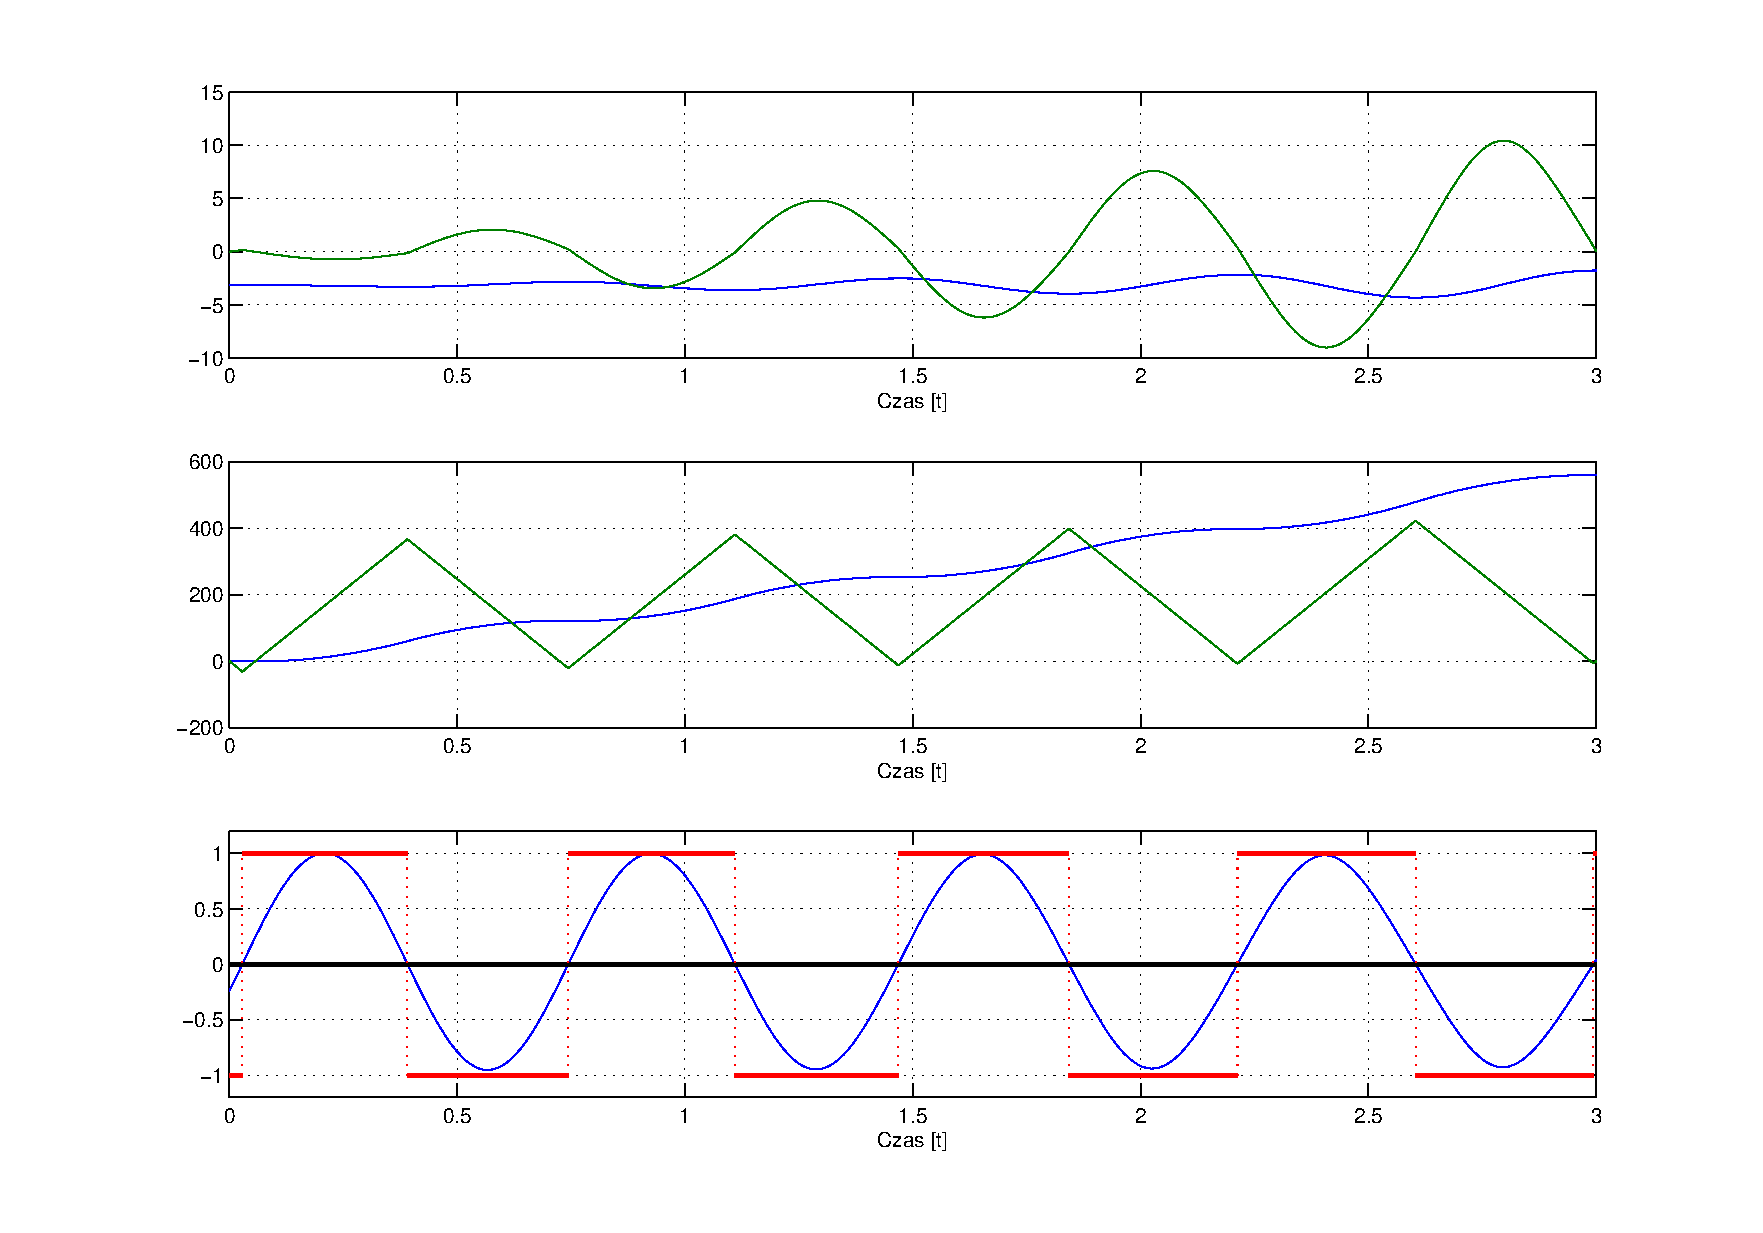
\includegraphics[viewport=81bp 414bp 811bp 599bp,clip,scale=0.65]{przebieg3s}} \\	
	\subfloat[Przebieg pozycji ({\color{matlabblue}niebieski}) oraz prędkości ({\color{matlabgreen}zielony}) wału]{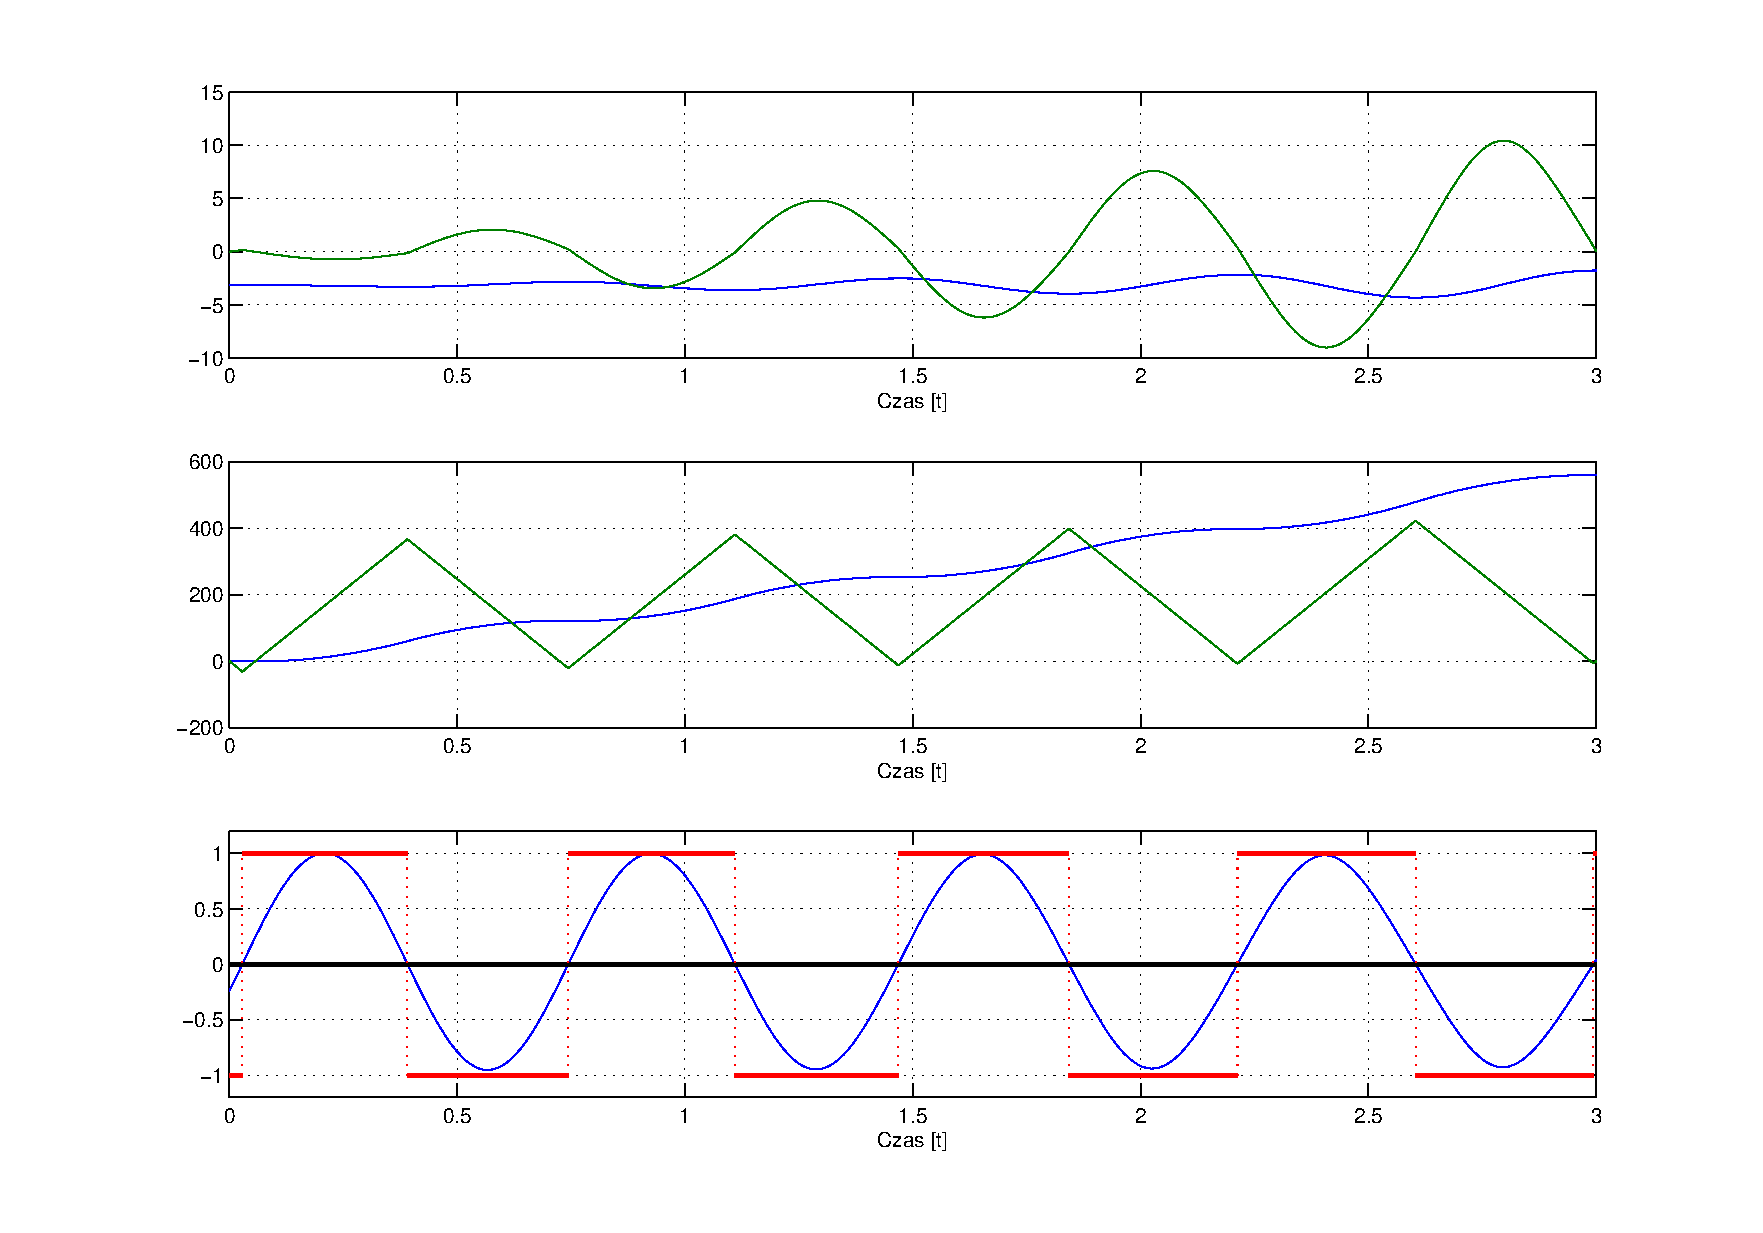
\includegraphics[viewport=81bp 217bp 811bp 414bp,clip,scale=0.65]{przebieg3s}} \\
	\subfloat[Przebieg funkcji przełączącej ({\color{matlabblue}niebieski}) oraz sterowania ({\color{matlabred}czerwony})]{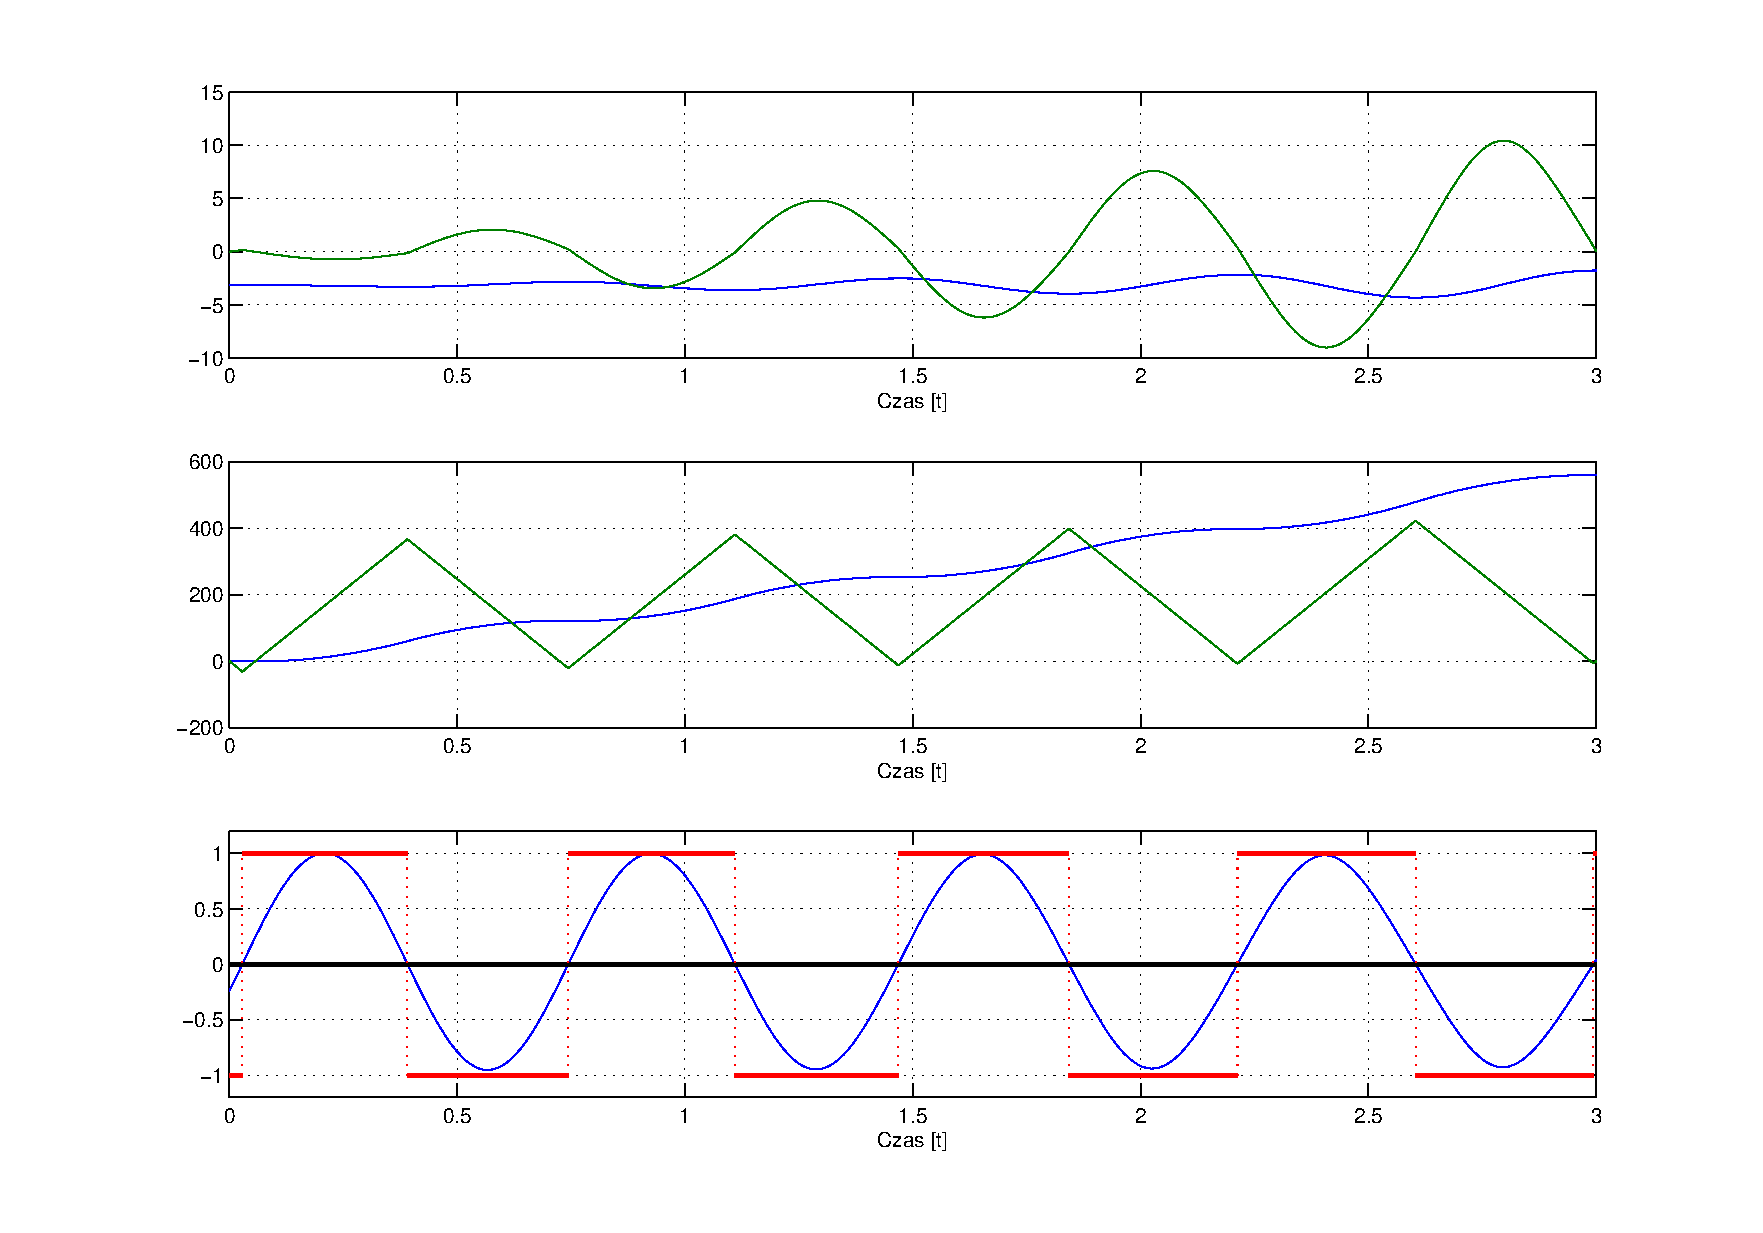
\includegraphics[viewport=81bp 38bp 811bp 217bp,clip,scale=0.65]{przebieg3s}}
	\caption{Przebiegi stanów dla $T=3$s.}
	\label{fig-ex1}
	\end{centering}
\end{figure}

\newpage

\begin{figure}[H]
	\begin{centering}
	\subfloat[Przebieg pozycji ({\color{matlabblue}niebieski}) oraz prędkości ({\color{matlabgreen}zielony}) wahadła]{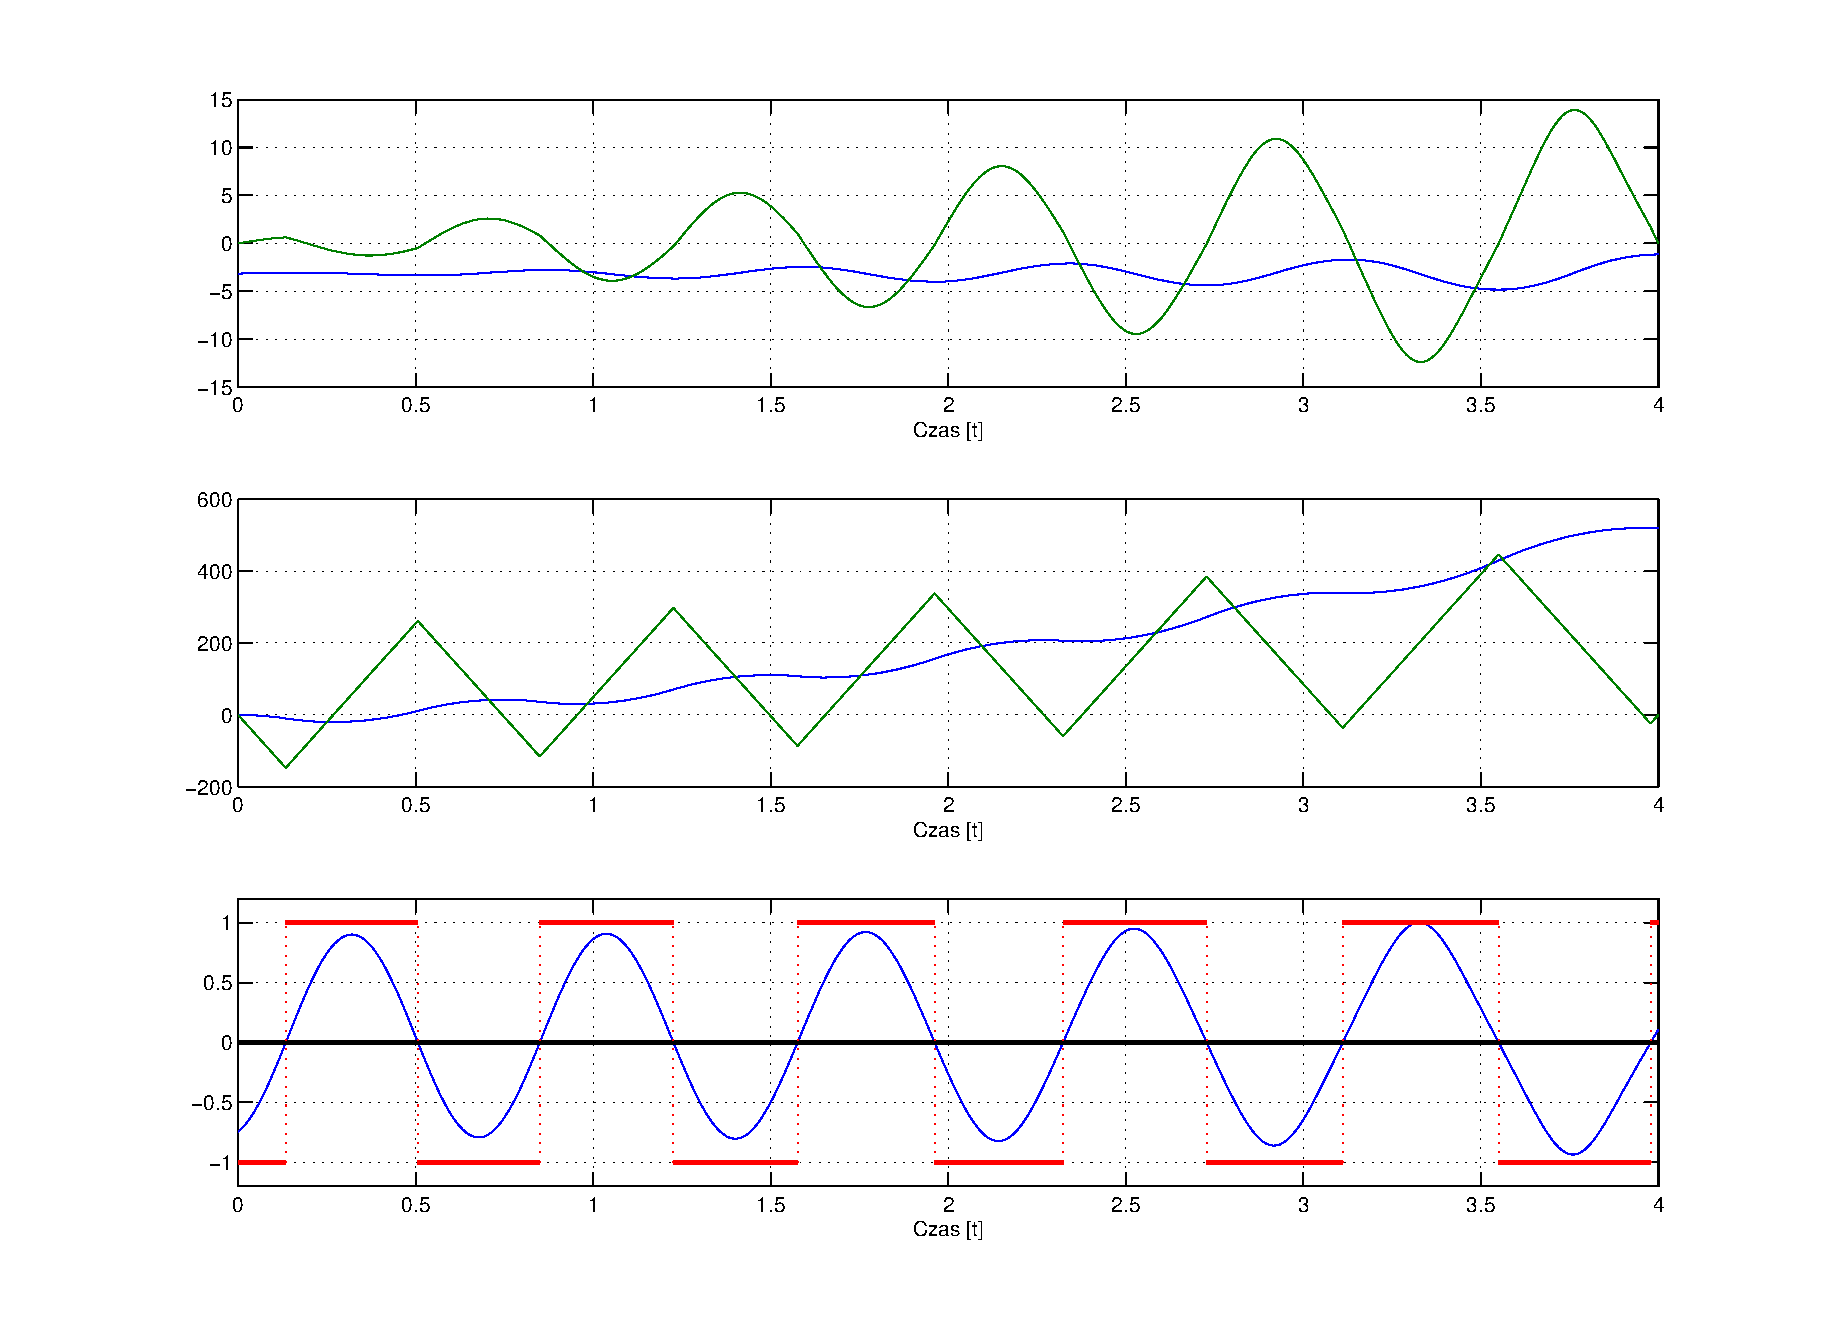
\includegraphics[viewport=81bp 414bp 811bp 599bp,clip,scale=0.65]{przebieg4s}} \\	
	\subfloat[Przebieg pozycji ({\color{matlabblue}niebieski}) oraz prędkości ({\color{matlabgreen}zielony}) wału]{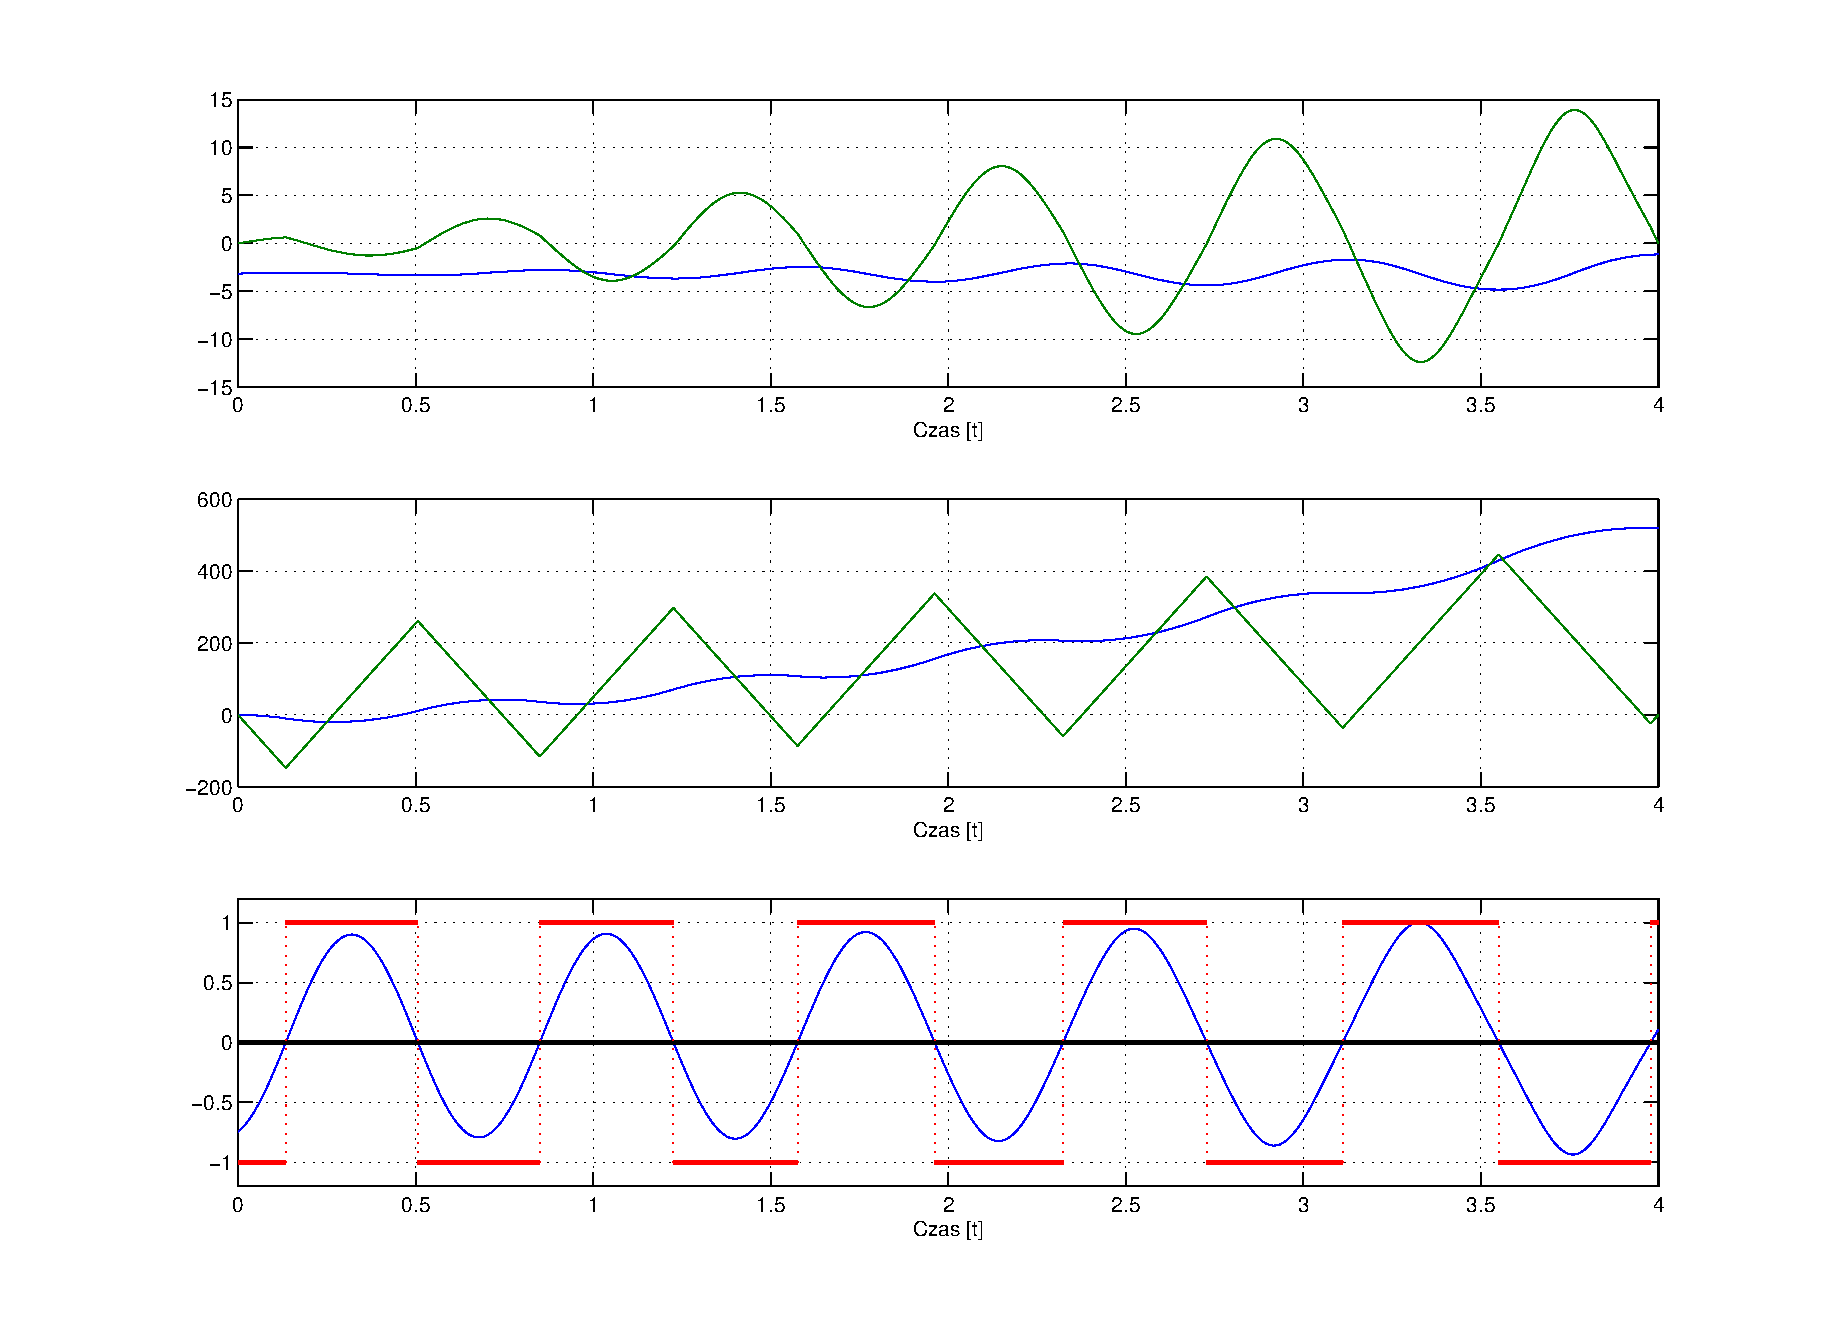
\includegraphics[viewport=81bp 217bp 811bp 414bp,clip,scale=0.65]{przebieg4s}} \\
	\subfloat[Przebieg funkcji przełączącej ({\color{matlabblue}niebieski}) oraz sterowania ({\color{matlabred}czerwony})]{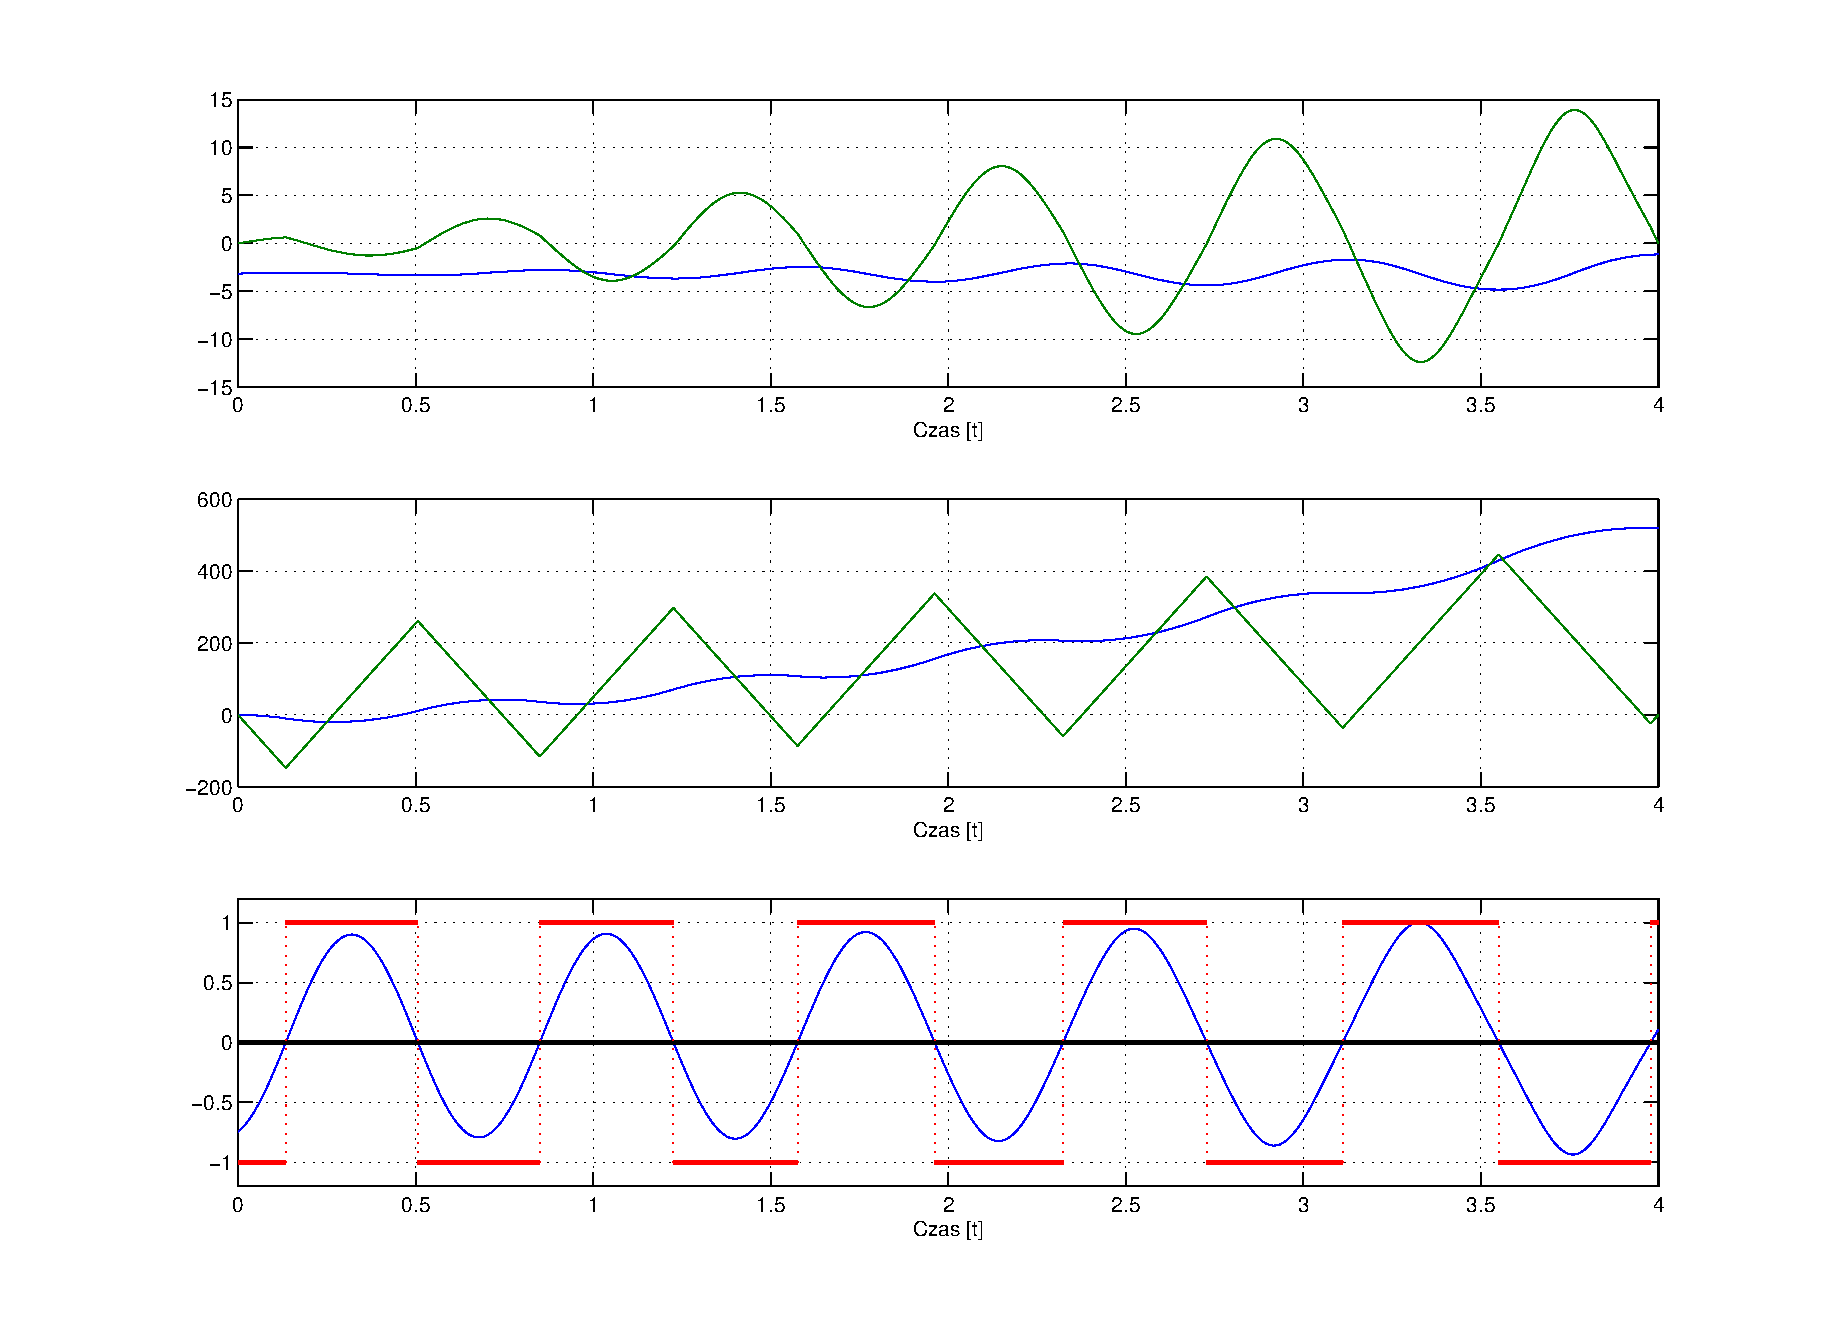
\includegraphics[viewport=81bp 38bp 811bp 217bp,clip,scale=0.65]{przebieg4s}}
	\caption{Przebiegi stanów dla $T=4$s.}
	\label{fig-ex2}
	\end{centering}
\end{figure}

\pagebreak
\section{Sterowanie czasooptymalne}

Ze zbioru rozwiązań optymalnych dla różnych horyzontów czasowych wybrano ten, który osiąga zadany stan końcowy z~dokładnością do $10^{-3}$ w najkrótszym czasie (Rys.~\ref{fig-QT}). Odczytana wielkość horyzontu wyniosła $T=t_{f}=5.05s$, natomiast wartość pomocniczego wskaźnika jakości, określonego wzorem (\ref{eq-wskjakosci}) $Q_{T}=0.02645$. Przebieg sterowania czasoptymalnego oraz odpowiadających mu stanów systemu pokazano na rysunku~\ref{fig-czasooptymalny}.

\begin{figure}[ht]
	\begin{centering}
	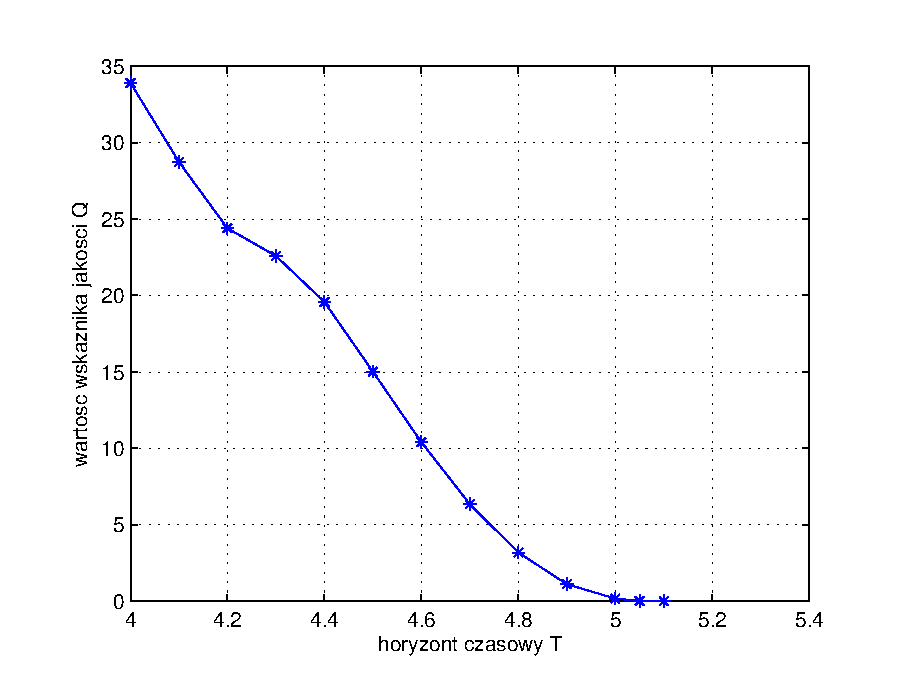
\includegraphics[scale=1.0]{QT}
	\caption{Zależność optymalnej wartości wskaźnika jakości od przyjętego horyzontu czasowego.}
	\label{fig-QT}
	\end{centering}
\end{figure}

\newpage

\begin{figure}[ht]
	\begin{centering}
	\subfloat[Przebieg pozycji ({\color{matlabblue}niebieski}) oraz prędkości ({\color{matlabgreen}zielony}) wahadła]{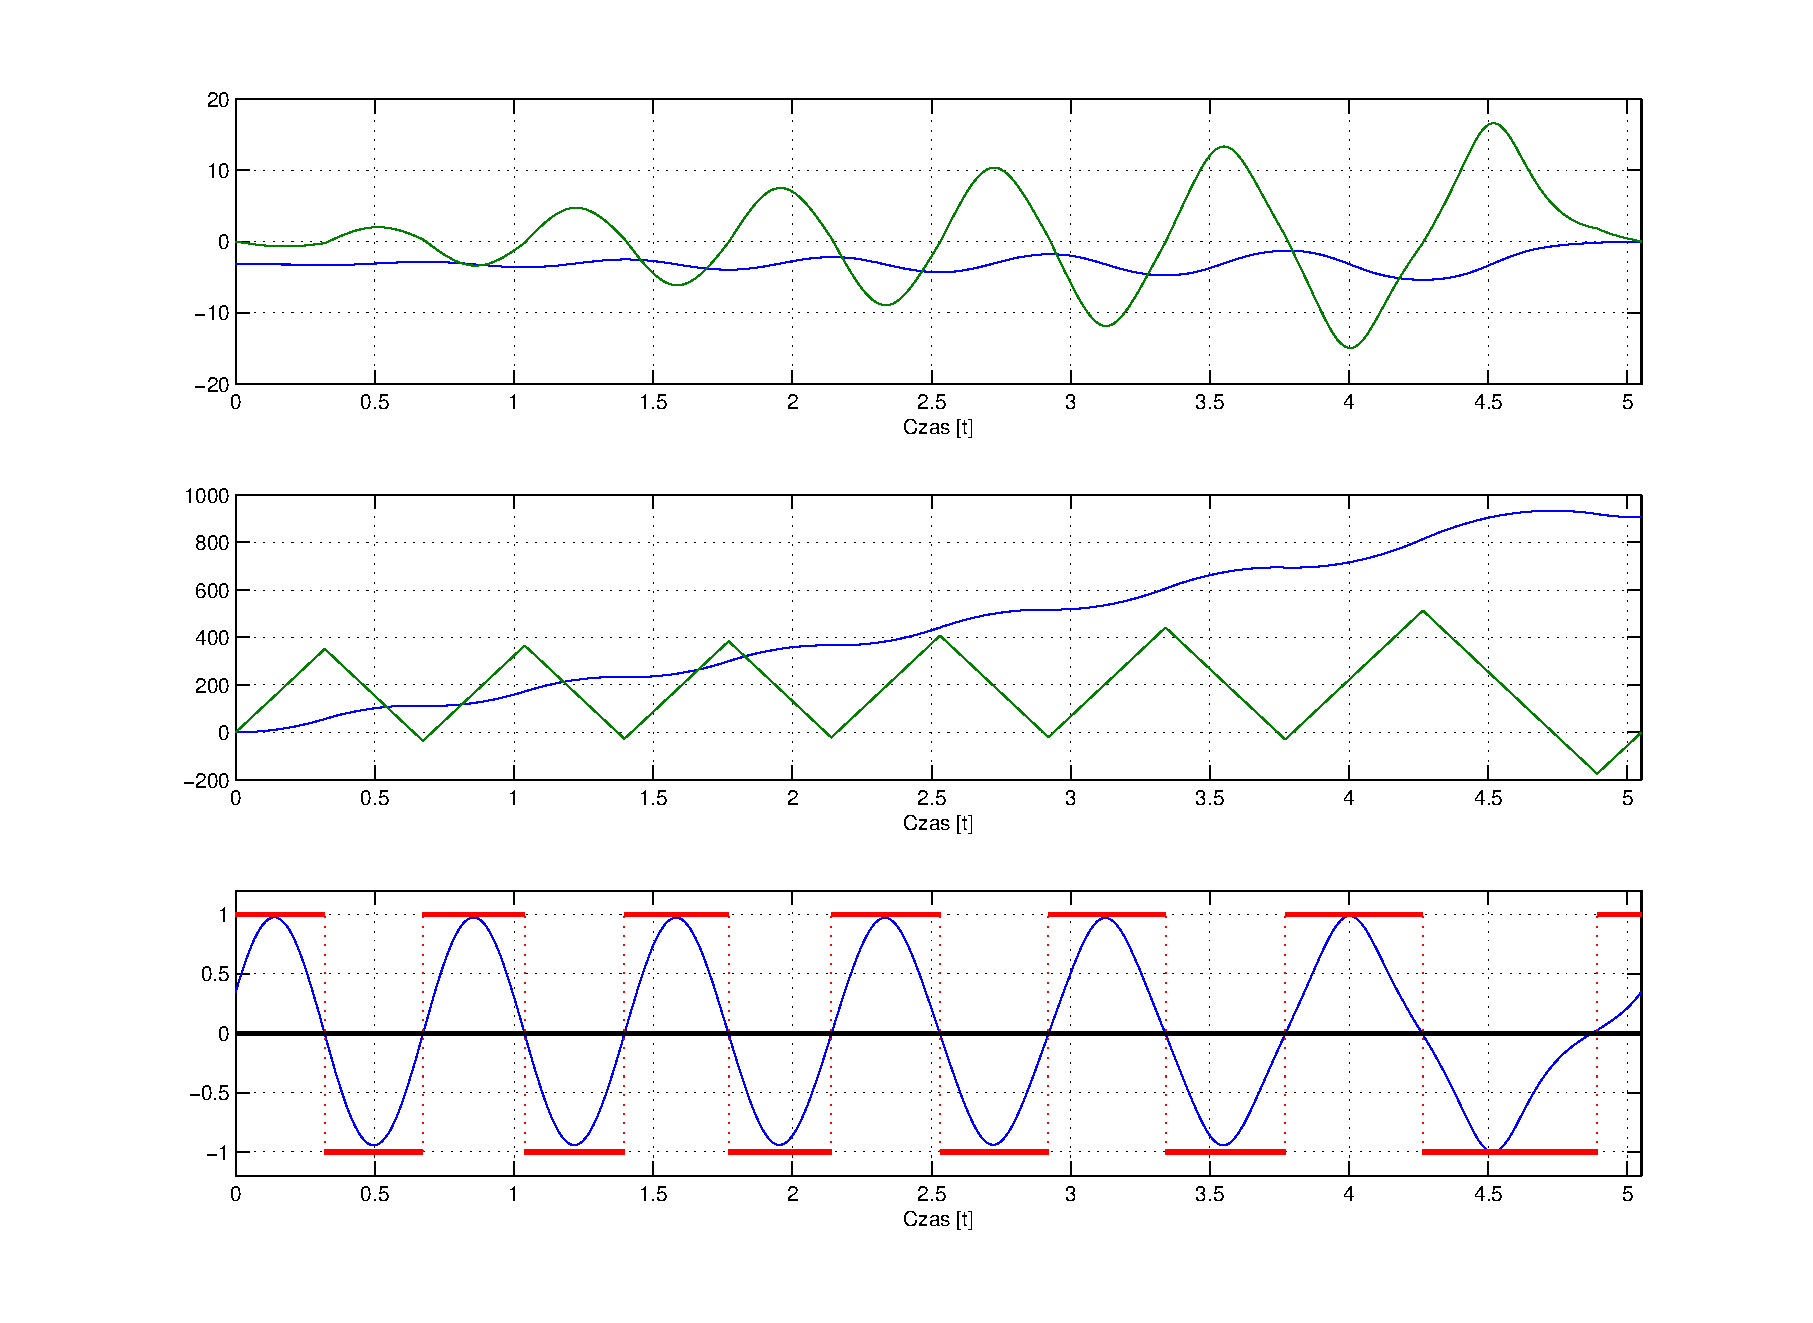
\includegraphics[viewport=81bp 414bp 811bp 599bp,clip,scale=0.65]{przebieg505s}} \\	
	\subfloat[Przebieg pozycji ({\color{matlabblue}niebieski}) oraz prędkości ({\color{matlabgreen}zielony}) wału]{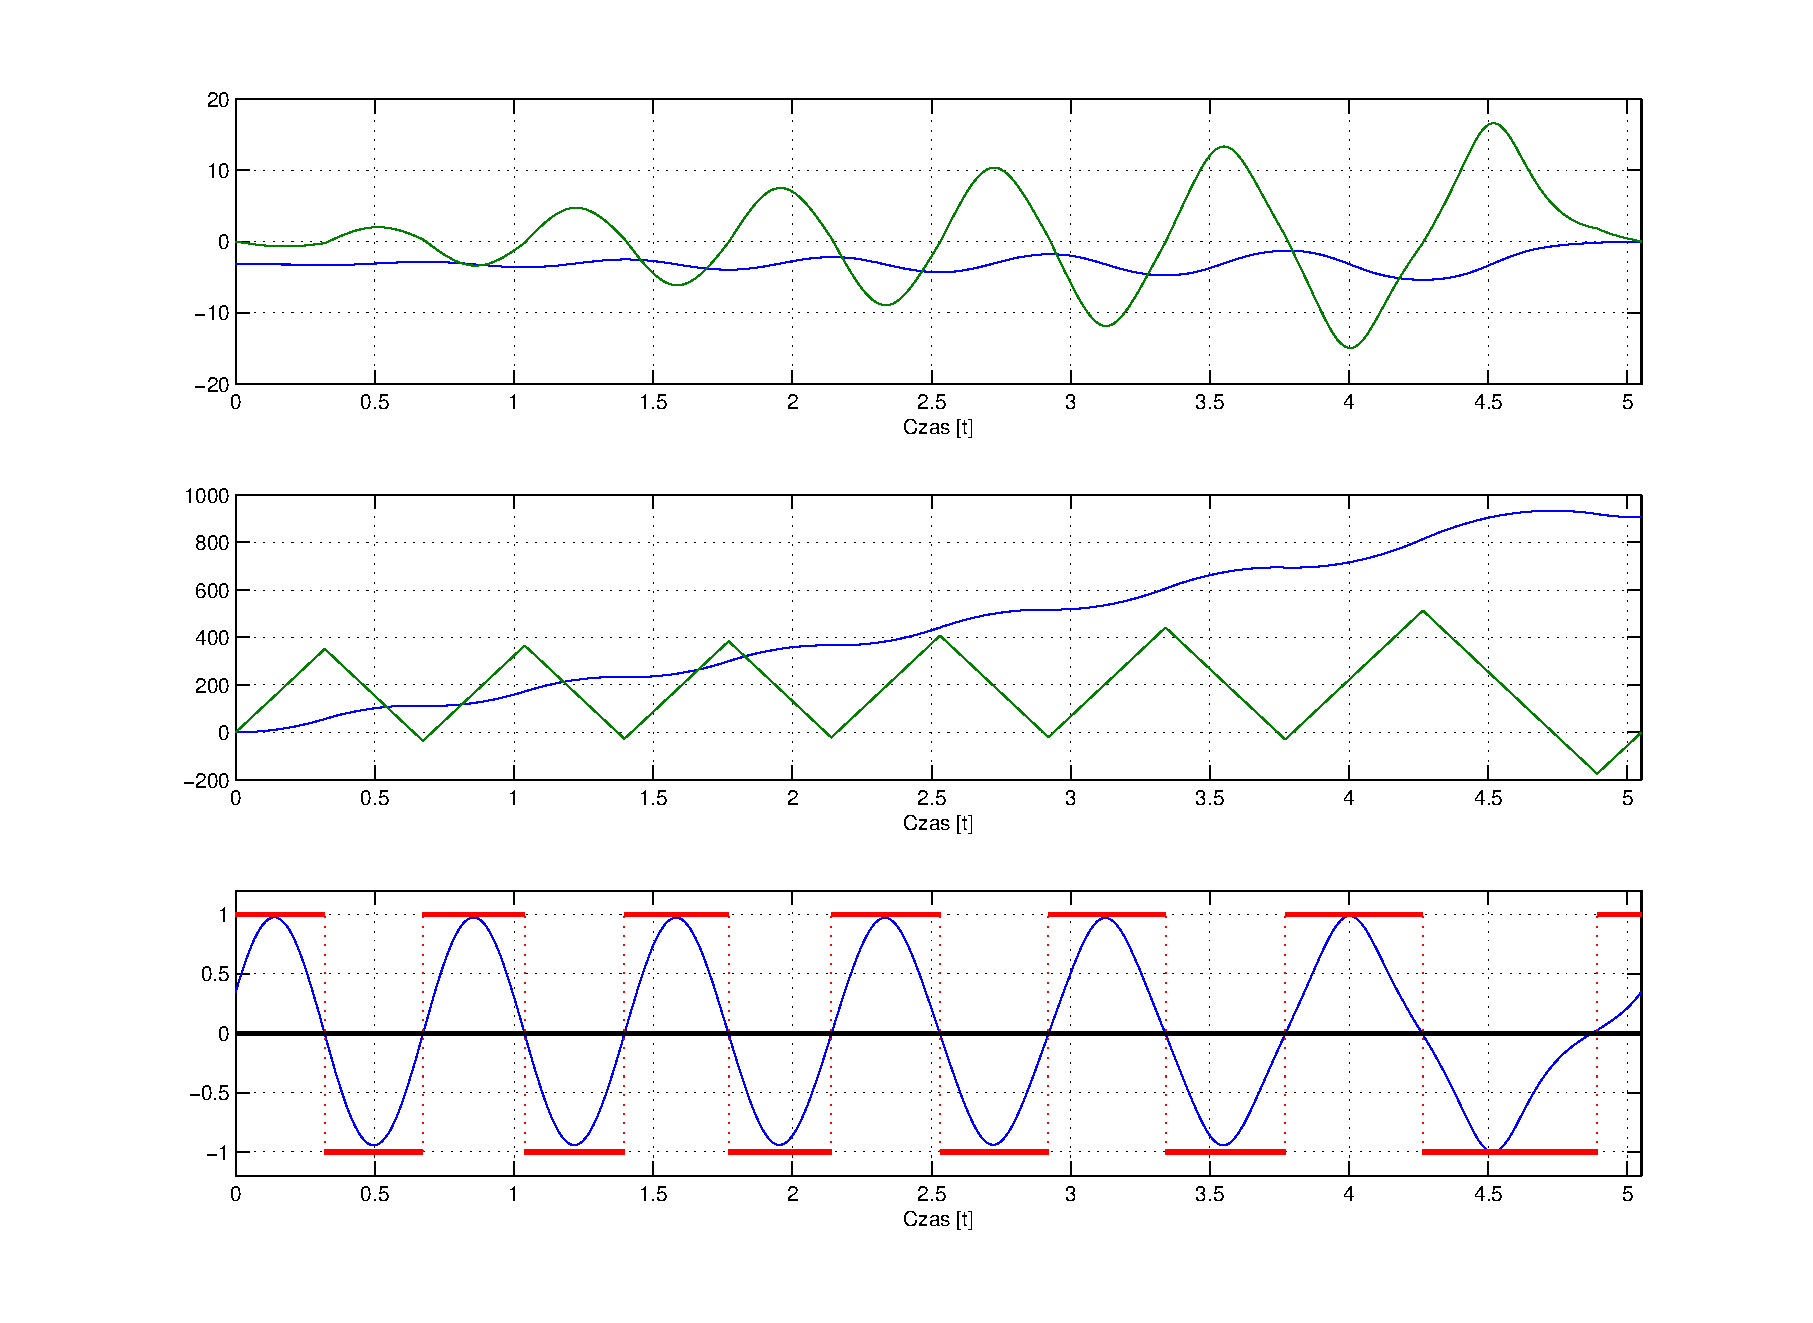
\includegraphics[viewport=81bp 217bp 811bp 414bp,clip,scale=0.65]{przebieg505s}} \\
	\subfloat[Przebieg funkcji przełączącej ({\color{matlabblue}niebieski}) oraz sterowania ({\color{matlabred}czerwony})]{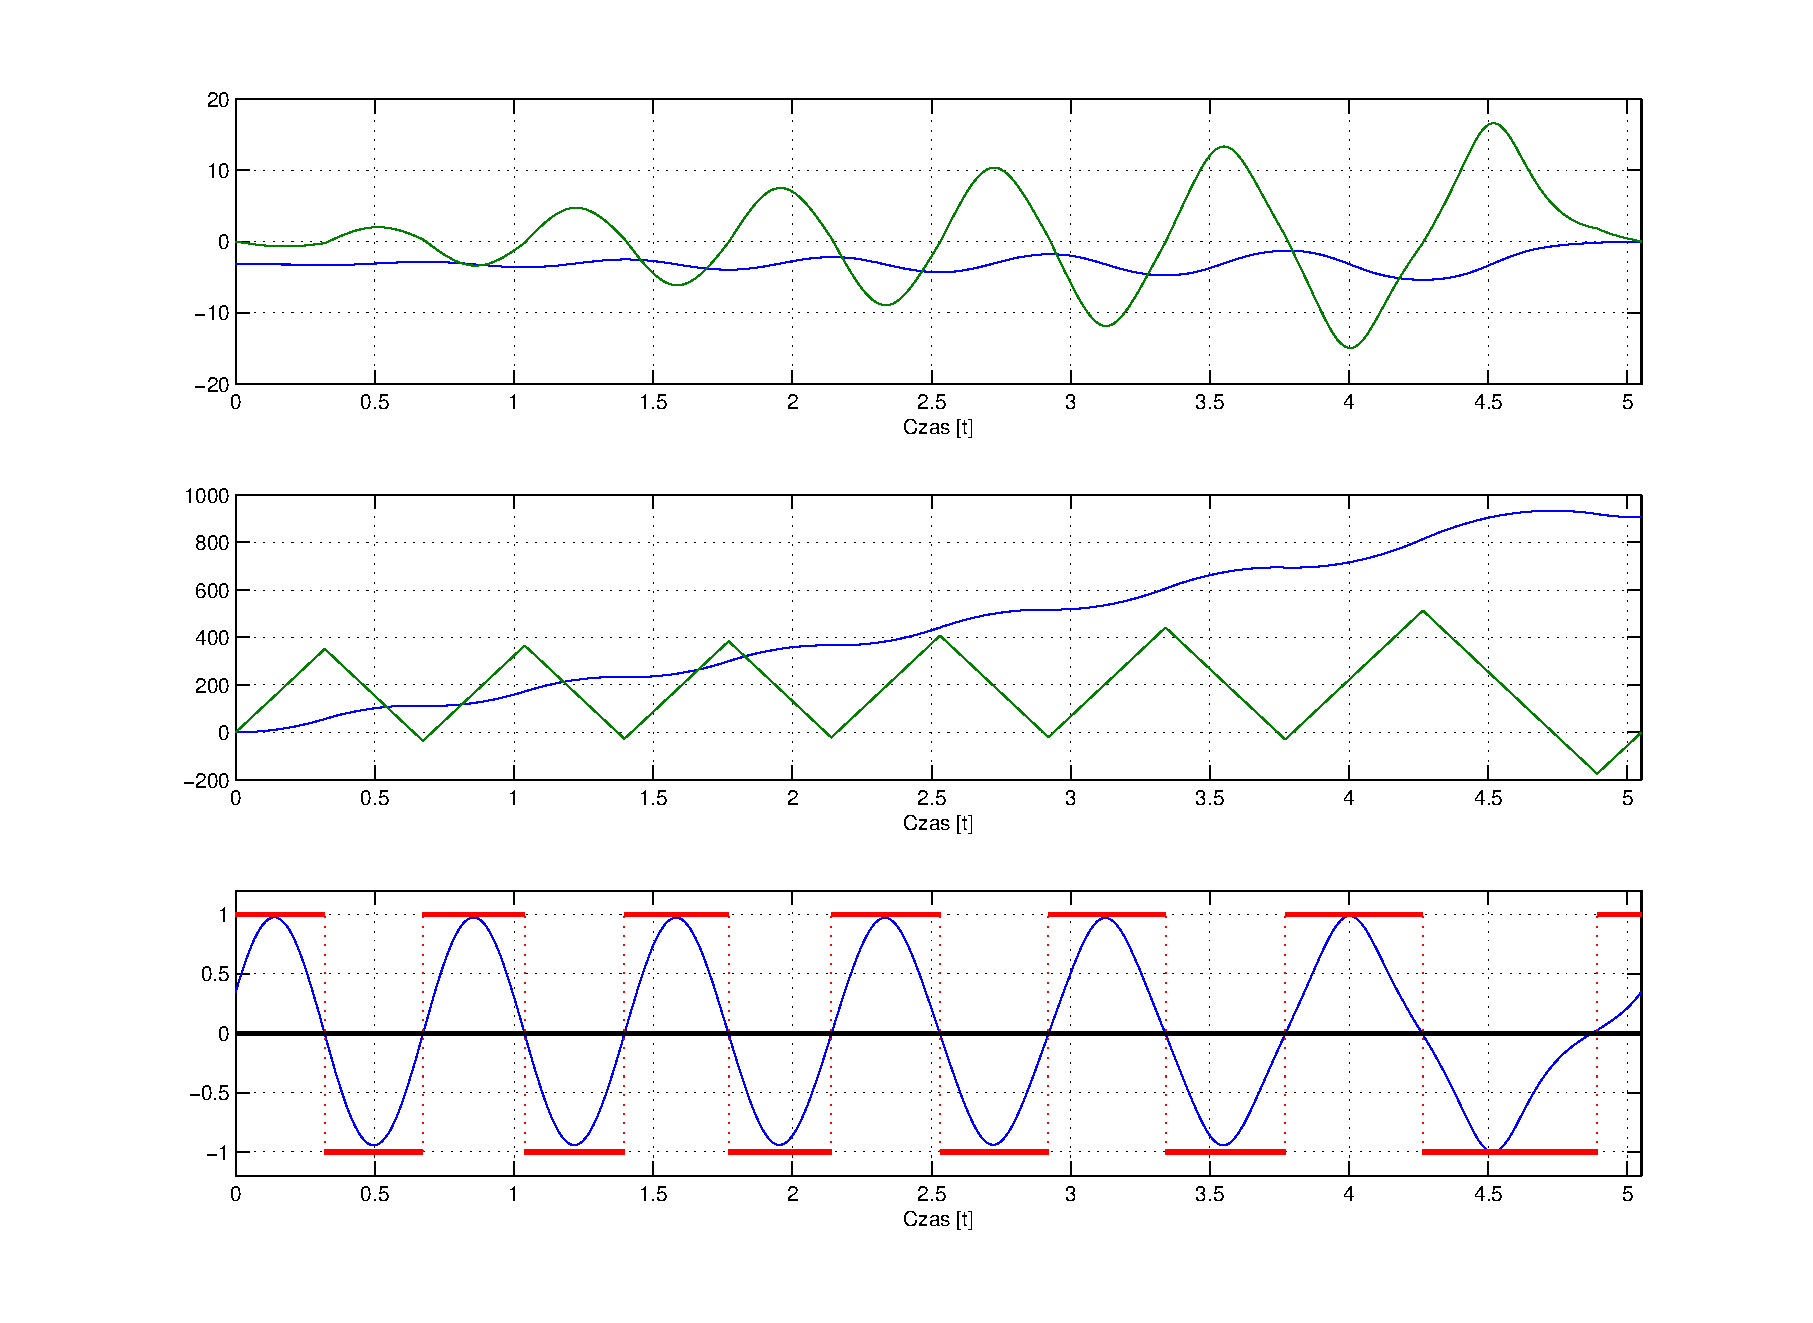
\includegraphics[viewport=81bp 38bp 811bp 217bp,clip,scale=0.65]{przebieg505s}}
	\caption{Przebiegi stanów dla $T=5.05$s.}
	\label{fig-czasooptymalny}
	\end{centering}
\end{figure}

\newpage
\phantomsection\addcontentsline{toc}{section}{\appendixname\ - Kod źródłowy}
\section*{\appendixname\ - Kod źródłowy}

\lstset{
	tabsize=2,
	basicstyle=\small\ttfamily, %\footnotesize
	numbers=left,
	numberstyle=\tiny,
	stepnumber=1, 
	numbersep=5pt,
	aboveskip={1.5\baselineskip},
	columns=fixed,
	extendedchars=true,
	breaklines=true,
	prebreak = \raisebox{0ex}[0ex][0ex]{\ensuremath{\hookleftarrow}},
	frame=single,
	showtabs=false,
	showspaces=false,
	showstringspaces=false,
	keywordstyle=[1]\color[rgb]{0.00,0.0,0.78},
	commentstyle=\color[rgb]{0.0, 0.56, 0.16},
	stringstyle=\color[rgb]{0.69,0.25,1.0},
	language=Matlab
}

{\renewcommand{\baselinestretch}{1.05}
\lstinputlisting[title=\texttt{bfgs.m} - główny plik]{../bfgs.m}
\lstinputlisting[title=\texttt{comodel.m} - prawa strona rówania sprzężonego]{../comodel.m}
\lstinputlisting[title=\texttt{model.m} - prawa strona rówania stanu]{../model.m}
\lstinputlisting[title=\texttt{switching\_fun.m} - funkcja przełączająca]{../switching_fun.m}
\lstinputlisting[title=\texttt{costfun.m} - funkcjonał jakości]{../costfun.m}
\lstinputlisting[title=\texttt{divdiff.m} - weryfikacja poprawności obliczania pochodnych]{../divdiff.m}
\lstinputlisting[title=\texttt{linesearch.m} - poszukiwanie na kierunku]{../linesearch.m}
\lstinputlisting[title=\texttt{reduction.m} - redukcja czasów przełączeń]{../reduction.m}
\lstinputlisting[title=\texttt{gradient.m} - pochodna funkcjonału jakości względem czasów przełączeń]{../gradient.m}
\lstinputlisting[title=\texttt{rk4.m} - solver dla równań stanu]{../rk4.m}
\lstinputlisting[title=\texttt{rk4r.m} - solver dla równań sprzężonych]{../rk4r.m}
\lstinputlisting[title=\texttt{uranges.m} - generuje przedziały sterowania]{../uranges.m}
\lstinputlisting[title=\texttt{plotcharts.m} - plotowanie wykresów]{../plotcharts.m}
}

\end{document}
